% ============================================================================
% AOGS GUIDEBOOK — the complete, teach-from-zero companion to the poster.
% Explains every mechanism in full: the thermal engine, the shadowing
% ray-casting algorithm (step by step, with a worked ray), the density grid
% and its justification, the two branches, the degeneracy, the retrieval and
% the statistics. Numbers via poster_numbers.tex (generated).
% Build:  /Library/TeX/texbin/pdflatex aogs_guidebook.tex   (x2)
% ============================================================================
\documentclass[11pt]{article}
\usepackage[a4paper, margin=20mm]{geometry}
\usepackage[T1]{fontenc}
\usepackage{newtxtext,newtxmath}
\usepackage{graphicx}
\usepackage{booktabs}
\usepackage{xcolor}
\usepackage[font=small,labelfont=bf]{caption}
\usepackage{enumitem}
\usepackage{amsmath}
\usepackage{mdframed}
\usepackage{float}
\usepackage[hidelinks]{hyperref}
\newcommand{\horAfif}{14.0}
\newcommand{\lossAfif}{1.16}
\newcommand{\svfAfif}{0.985}
\newcommand{\kdstarAfif}{4.60}
\newcommand{\horAsev}{10.1}
\newcommand{\lossAsev}{0.18}
\newcommand{\svfAsev}{0.991}
\newcommand{\kdstarAsev}{7.08}
\newcommand{\rmsehayAfif}{2.03}
\newcommand{\rmsecpAfif}{1.74}
\newcommand{\bestzcpAfif}{5/30}
\newcommand{\bestrhocpAfif}{1500/1700/1700}
\newcommand{\rmsecKAfif}{0.90}
\newcommand{\bestzcKAfif}{10/30}
\newcommand{\bestrhocKAfif}{1500/1700/1800}
\newcommand{\rmsehayAsev}{0.54}
\newcommand{\rmsecpAsev}{0.39}
\newcommand{\bestzcpAsev}{5/30}
\newcommand{\bestrhocpAsev}{1500/1700/1700}
\newcommand{\rmsecKAsev}{0.36}
\newcommand{\bestzcKAsev}{5/30}
\newcommand{\bestrhocKAsev}{1300/1500/1900}
\newcommand{\rmsehomAfif}{2.31}
\newcommand{\rmsehomAsev}{3.76}
\newcommand{\xferatAsev}{1.64}
\newcommand{\xferatAfif}{1.73}
\newcommand{\svfdtirAfif}{1.15}
\newcommand{\svfdtallAfif}{1.30}
\newcommand{\svfdtirAsev}{0.65}
\newcommand{\svfdtallAsev}{0.74}
\newcommand{\shadowcoolAfif}{2.22}
\newcommand{\shadowcoolAsev}{0.48}
\newcommand{\stabcKAfif}{13}
\newcommand{\bootcicKAfif}{0.26--1.08}
\newcommand{\stabcKAsev}{36}
\newcommand{\bootcicKAsev}{0.25--0.43}
\newcommand{\driftmax}{35}
\newcommand{\closurewin}{0.70}


\definecolor{teal}{HTML}{2A6478}
\definecolor{coral}{HTML}{B85B3A}
\definecolor{forest}{HTML}{3D6E4A}
\definecolor{char}{HTML}{2A2520}
\definecolor{gridc}{HTML}{E8E5E0}
\definecolor{dim}{HTML}{8A857E}
\color{char}
\graphicspath{{../figures/poster/}{../figures/diagrams/}{../figures/explainers/}}
\setlist[itemize]{leftmargin=1.3em, itemsep=1pt, topsep=2pt}
\setlist[enumerate]{leftmargin=1.5em, itemsep=2pt, topsep=2pt}

\newcommand{\shead}[1]{\medskip\addcontentsline{toc}{section}{#1}%
  \noindent{\color{teal}\Large\bfseries #1}\par
  \nobreak\vspace{0pt}{\color{teal}\rule{\linewidth}{0.8pt}}\par\smallskip}
\newcommand{\sub}[1]{\medskip\addcontentsline{toc}{subsection}{#1}%
  \noindent{\color{char}\large\bfseries #1}\par\nobreak\smallskip}
% "intuition first" box
\newmdenv[linecolor=teal, linewidth=0.8pt, backgroundcolor=teal!6,
          roundcorner=3pt, innertopmargin=5pt, innerbottommargin=6pt,
          innerleftmargin=7pt, innerrightmargin=7pt, skipabove=5pt, skipbelow=4pt]{intuition}
% worked-example box
\newmdenv[linecolor=forest, linewidth=0.8pt, backgroundcolor=forest!5,
          roundcorner=3pt, innertopmargin=5pt, innerbottommargin=6pt,
          innerleftmargin=7pt, innerrightmargin=7pt, skipabove=5pt, skipbelow=4pt]{worked}
\newcommand{\intro}{\textbf{\color{teal}In plain words.}\ }
\newcommand{\workedhdr}{\textbf{\color{forest}Worked example.}\ }

\begin{document}

% ── COVER ────────────────────────────────────────────────────────────────────
\thispagestyle{empty}
\vspace*{2cm}
\begin{center}
{\Huge\bfseries A Guidebook to the}\\[6pt]
{\Huge\bfseries Discrete-Layer Lunar Thermal Study}\\[14pt]
{\large\color{teal}\bfseries Every mechanism, explained from the ground up ---\\
the thermal engine, the shadowing algorithm, the density grid, and the retrieval}\\[24pt]
{\large Ram\'on III P.\ Gregorio}\\[2pt]
{\normalsize Institute of Science Tokyo}\\[20pt]
{\footnotesize\color{dim} Companion to the AOGS poster \emph{Discrete Layer Thermal
Modeling of Lunar Landing Sites with Topographic Shadowing}.\\
Every physical value is drawn from the code and results archives; nothing is
typed from memory.}
\end{center}
\vfill
\begin{center}\footnotesize\color{dim}
How to read this book: each concept opens with a \textbf{plain-words} box, then the
full detail, then a \textbf{worked example} where numbers help. You can stop after
any box and still have understood the idea.
\end{center}
\clearpage

\tableofcontents
\clearpage

% ════════════════════════════════════════════════════════════════════════════
\shead{1\enspace The question, and the two advances}

\sub{1.1\enspace What Apollo measured, and why it still matters}
In 1971 and 1972, the Apollo 15 and 17 crews drilled boreholes and lowered strings
of thermometers 1--2.5 m into the lunar regolith. Over the following years those
sensors recorded the only \emph{in-situ} measurements of how heat flows out of the
Moon's interior --- the Heat Flow Experiment (HFE). From the temperature gradient
with depth and an estimate of the regolith's thermal conductivity, one recovers the
\textbf{geothermal heat flux} $Q_b$ and, with it, clues about the Moon's radioactive
inventory and thermal evolution. Fifty years later these two boreholes remain the
\emph{only} ground truth we have for the lunar subsurface thermal state.

\begin{intuition}
\intro The Moon is a slow oven leaking heat from the inside. Apollo put two
thermometers deep enough to feel that leak. If you know how well the regolith
conducts heat, the temperature rise with depth tells you how much heat is leaking.
This study is about pinning down that ``how well it conducts'' --- which turns out
to be inseparable from \emph{how dense} the regolith is.
\end{intuition}

\sub{1.2\enspace The parent result and what this study adds}
A prior study (``the letter'') fixed the regolith \emph{density} to a standard
model and retrieved one deep conductivity $K_d^{\star}$ per site:
$K_d^{\star}(\mathrm{A15})=\kdstarAfif$ and $K_d^{\star}(\mathrm{A17})=\kdstarAsev$
mW\,m$^{-1}$K$^{-1}$. This study keeps the same certified physics engine and asks a
complementary question --- \emph{what layered density structure best explains the
same temperatures?} --- while adding a second piece of physics the standard picture
ignores: the shadow the surrounding terrain casts on each site. So there are two
advances:
\begin{enumerate}
  \item \textbf{Topographic shadowing} (Part~III): the real skyline of hills and
    massifs around each borehole blocks part of the sunlight, computed by
    ray-tracing a digital elevation model.
  \item \textbf{Discrete density layers} (Part~IV): instead of one smooth density
    curve, a three-layer staircase whose depths and densities are swept and scored
    against the sensors.
\end{enumerate}
Figure~\ref{fig:schematic} is the whole idea in one picture; the pipeline that turns
it into numbers is Figure~\ref{fig:pipeline}.

\begin{figure}[H]\centering
  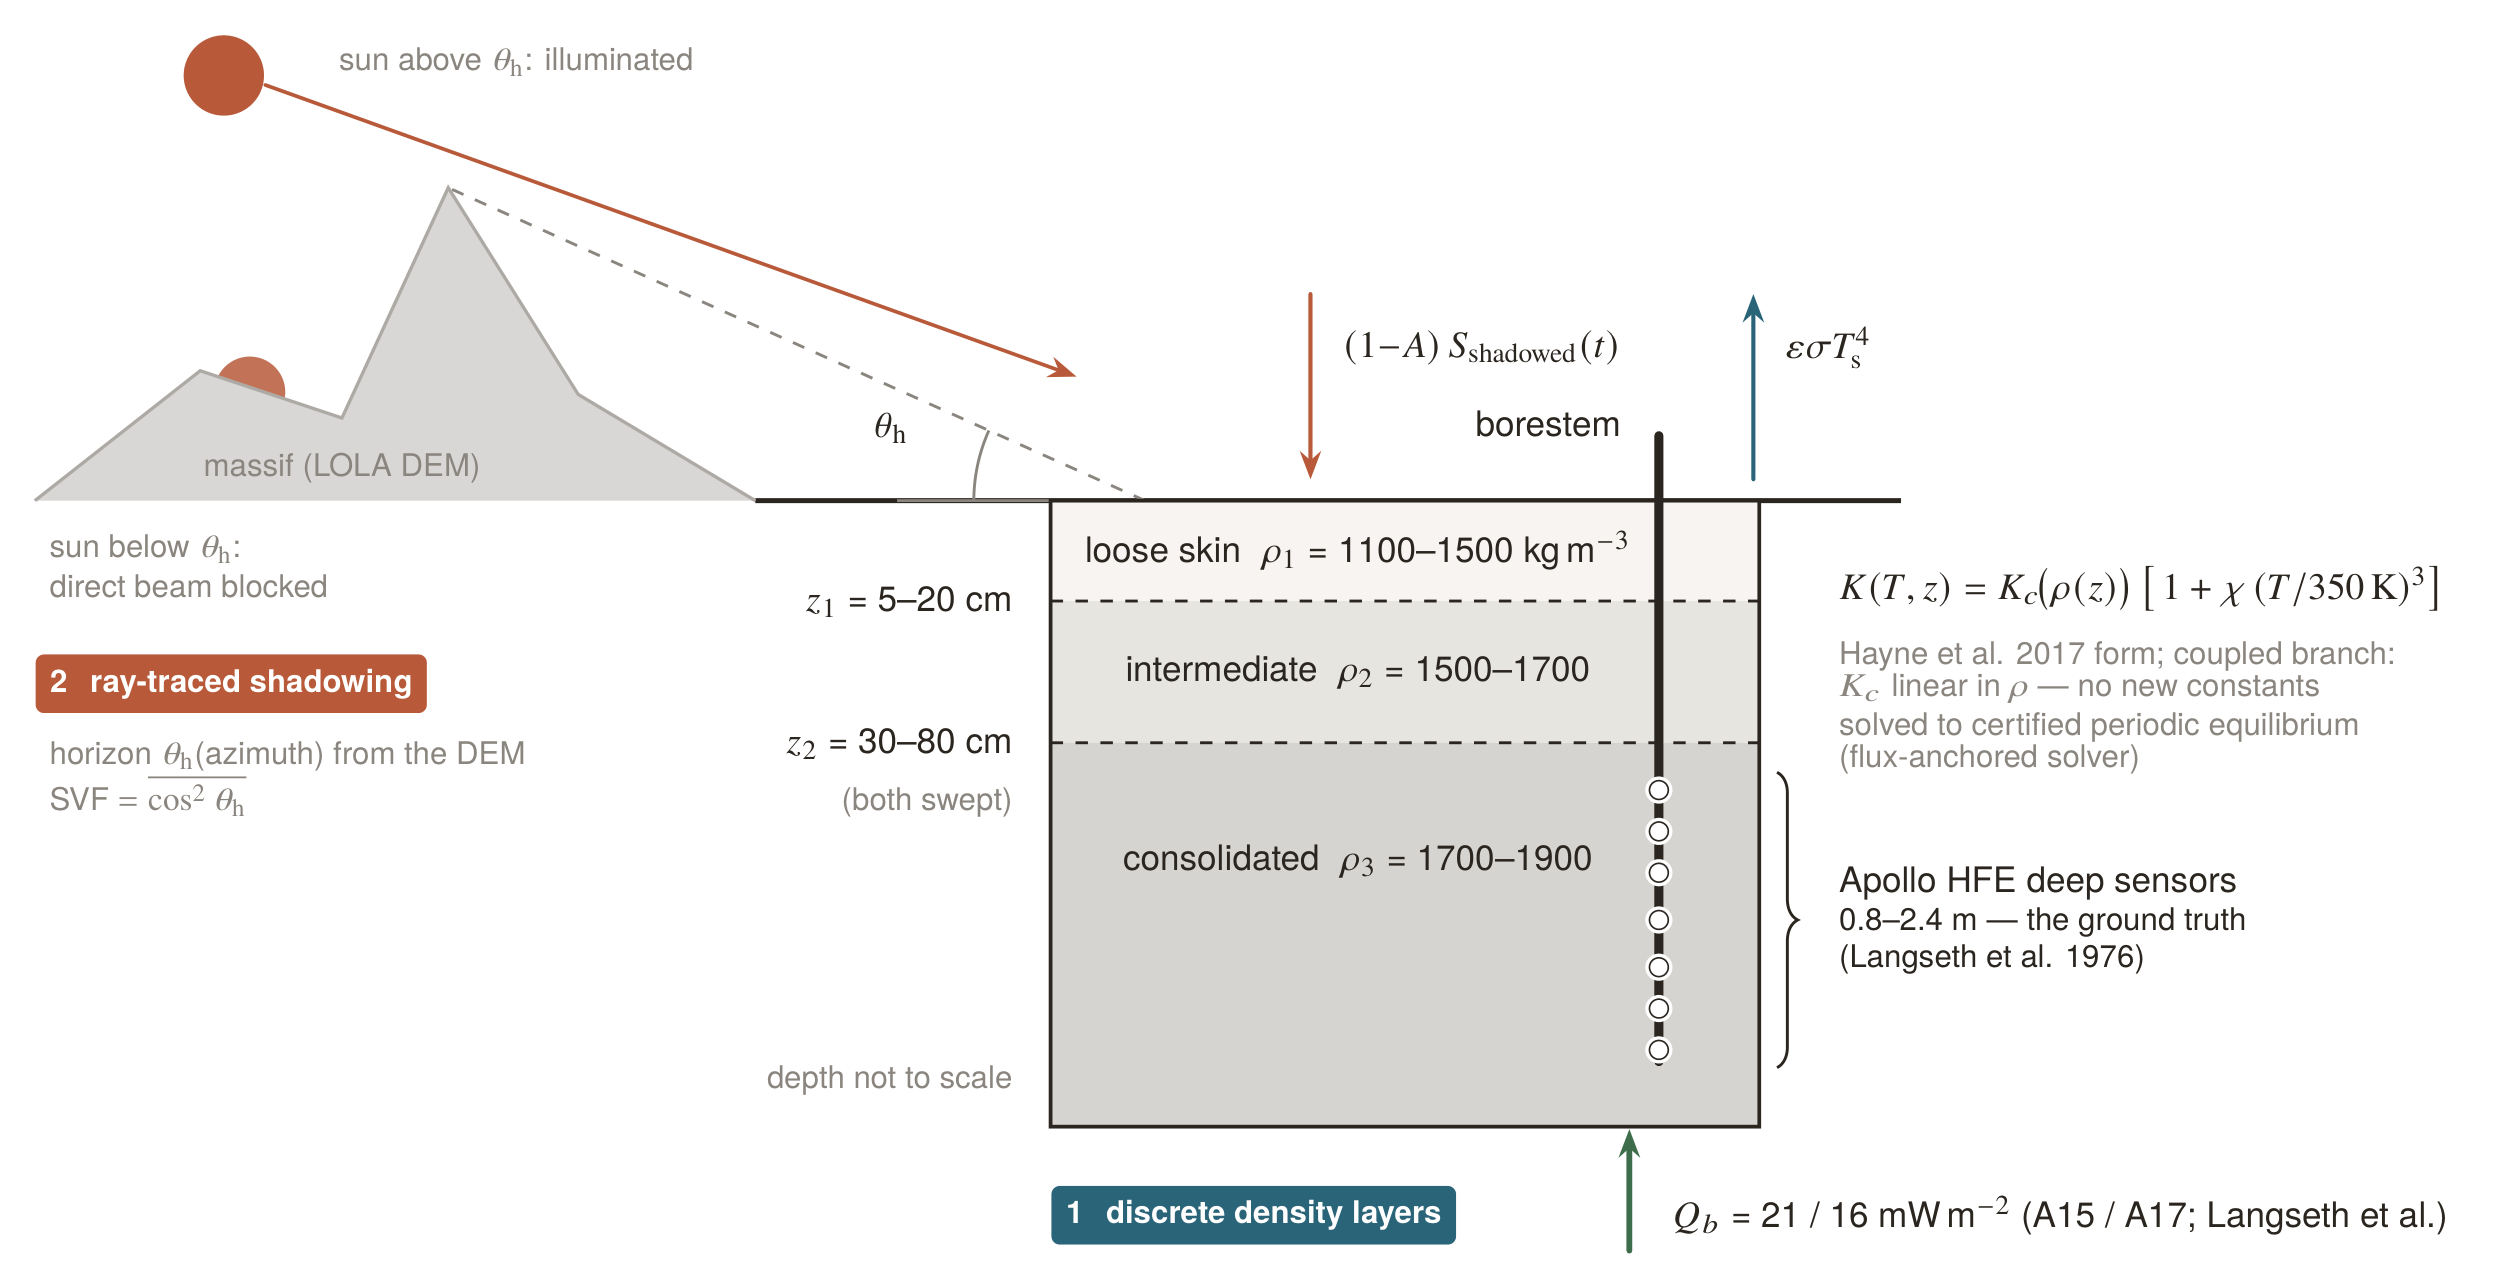
\includegraphics[width=0.86\linewidth]{aogs_model_schematic.pdf}
  \caption{The physical model. A three-layer regolith column (loose skin $\to$
  intermediate $\to$ consolidated) under sunlight that the terrain (left) can block.
  Fluxes: absorbed sunlight in, thermal emission out, geothermal $Q_b$ up from below.
  The two tagged items --- discrete layers and ray-traced shadowing --- are this
  study's additions; everything else is the certified baseline.}
  \label{fig:schematic}
\end{figure}

\begin{figure}[H]\centering
  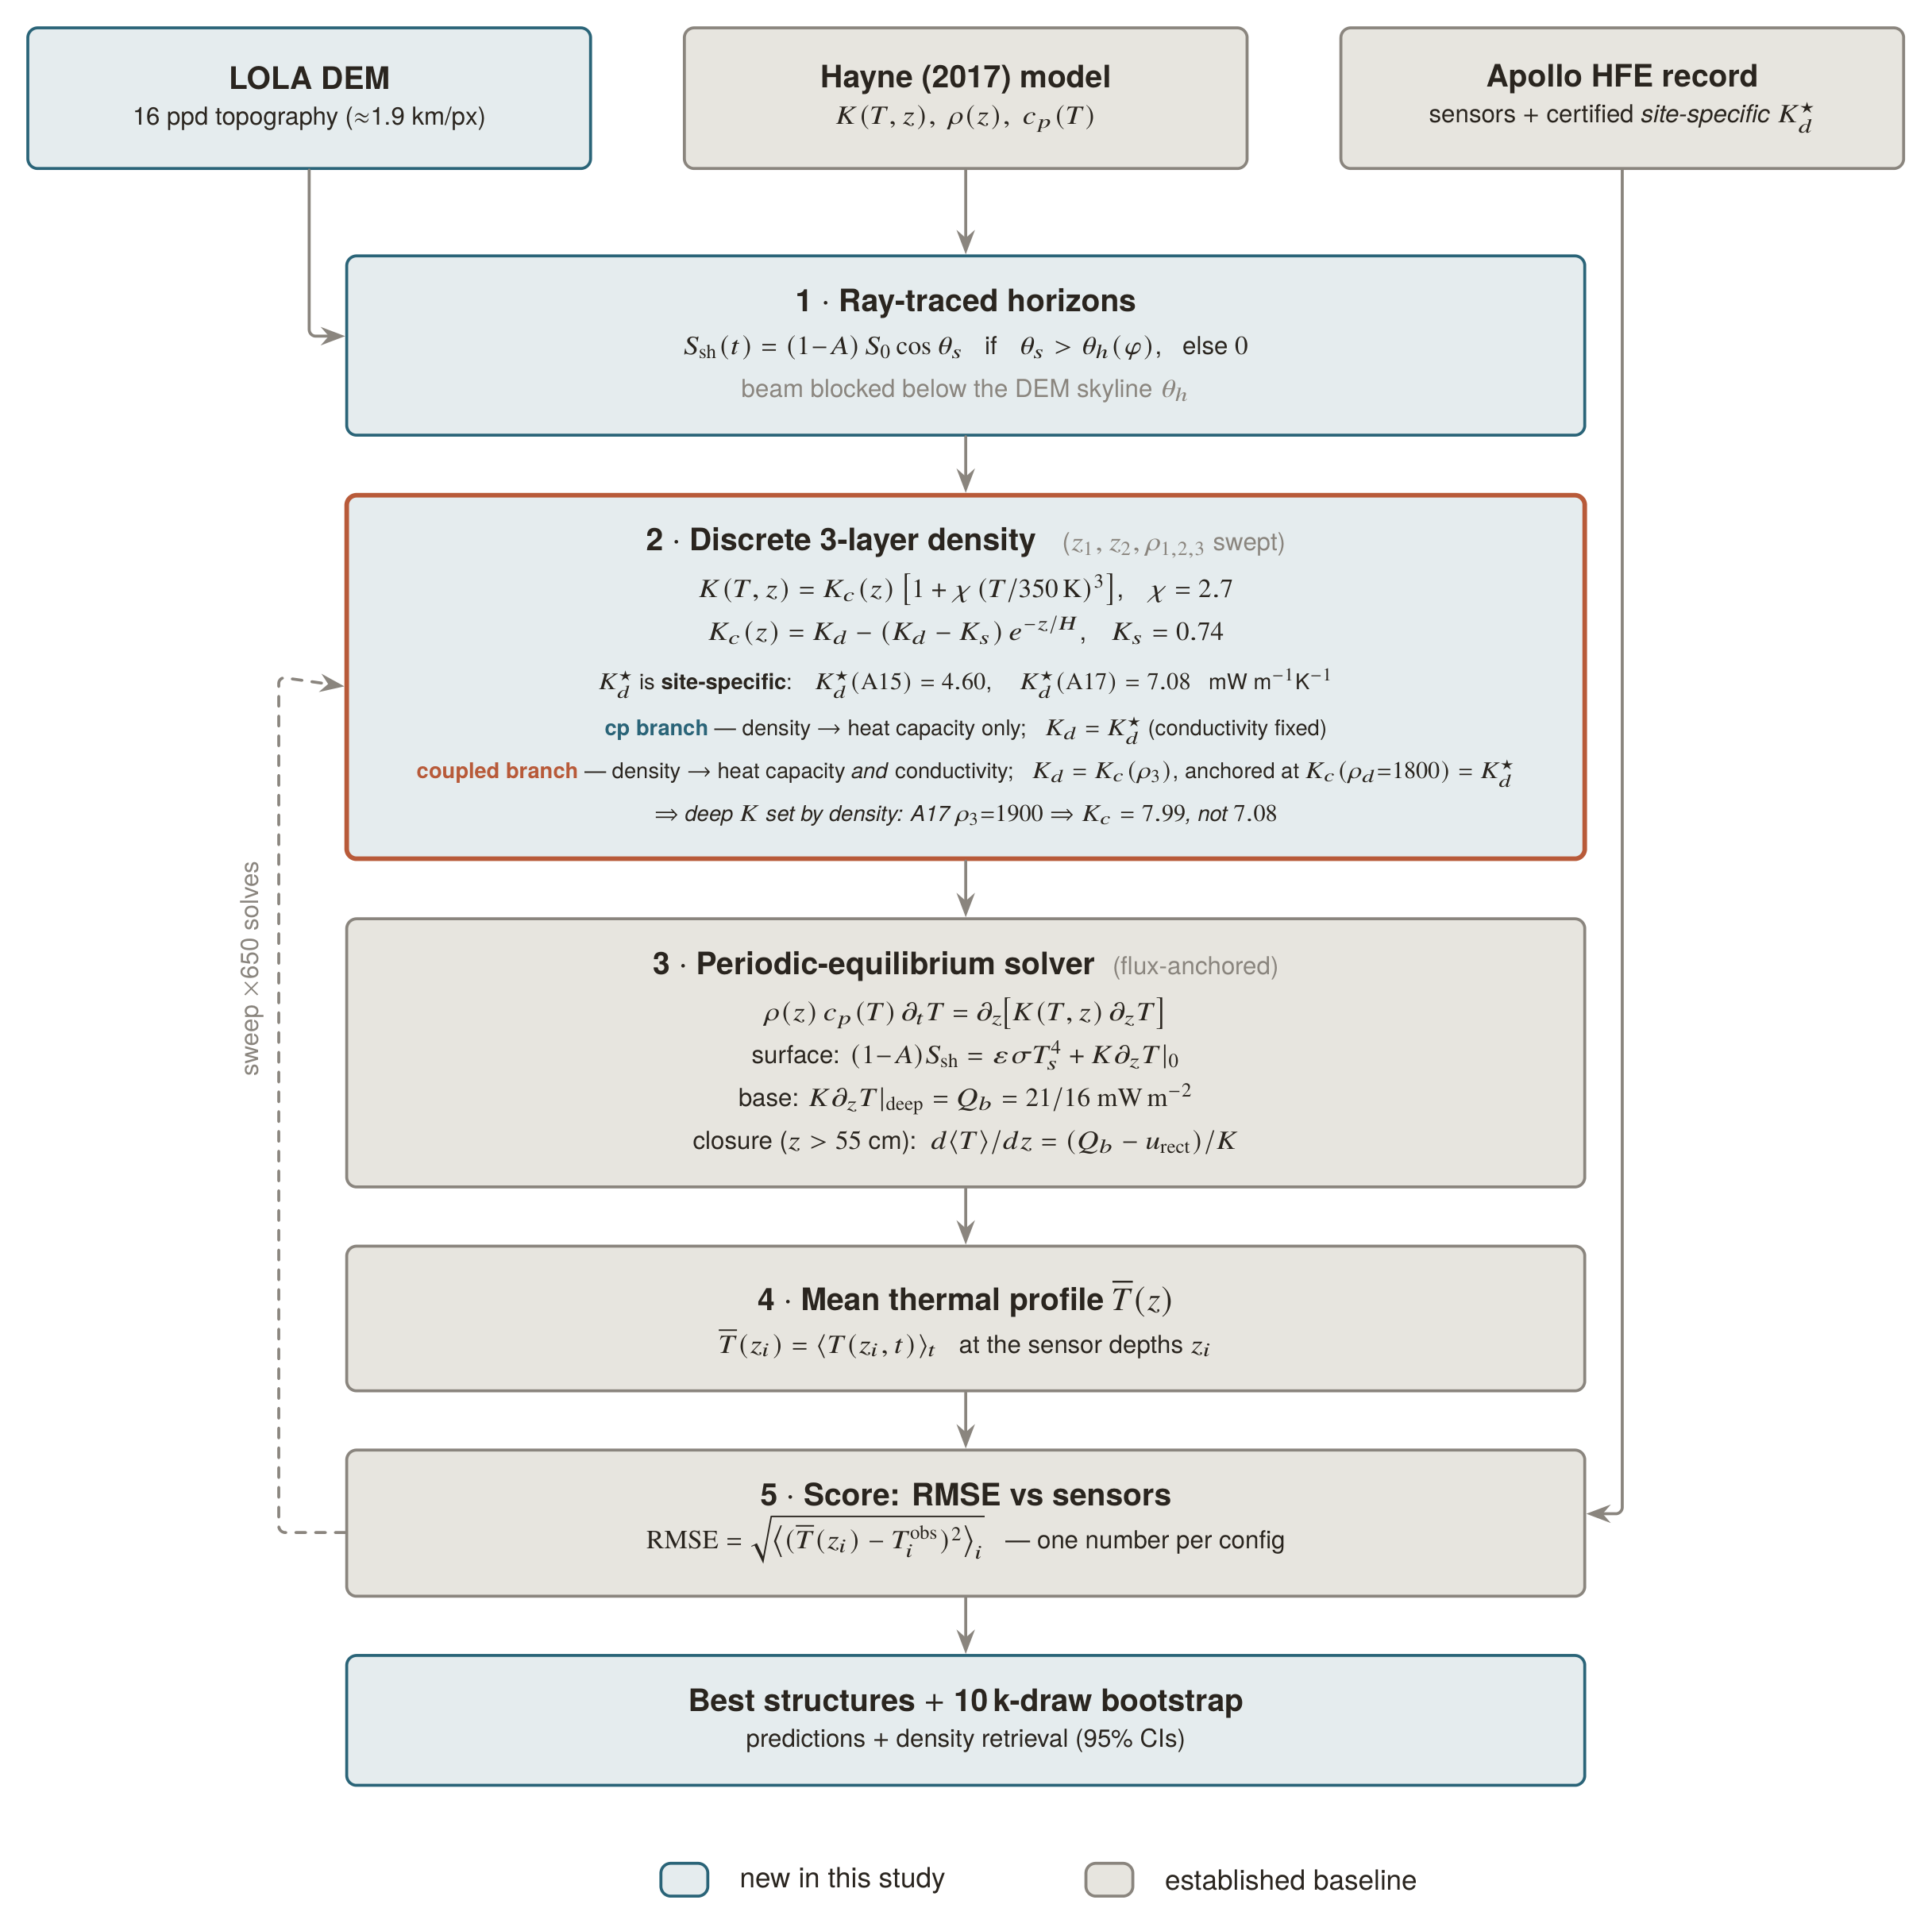
\includegraphics[width=0.66\linewidth]{aogs_pipeline_flowchart.pdf}
  \caption{The pipeline. Three inputs (LOLA DEM, Hayne model, Apollo record) feed a
  five-step chain --- ray-traced horizons $\to$ 3-layer density $\to$
  periodic-equilibrium solver $\to$ mean profile $\to$ RMSE --- looped over 650
  configurations. Teal boxes are new in this study; grey are the certified baseline.
  The equations in each box are the ones derived through this guidebook.}
  \label{fig:pipeline}
\end{figure}

% ════════════════════════════════════════════════════════════════════════════
\shead{2\enspace The thermal engine (the certified baseline)}
Both advances plug into an existing, validated 1-D heat solver. To understand what
the shadowing and the layers \emph{do}, you first need to know what they plug into.

\sub{2.1\enspace Heat conduction in a column of regolith}
Regolith moves heat by conduction only (no air, no water, no convection). In one
vertical dimension, energy conservation gives the heat equation
\begin{equation}
  \rho(z)\,c_p(T)\,\frac{\partial T}{\partial t}
   \;=\; \frac{\partial}{\partial z}\!\left[K(T,z)\,\frac{\partial T}{\partial z}\right],
  \label{eq:heat}
\end{equation}
where $T(z,t)$ is temperature, $\rho$ is density, $c_p$ is specific heat capacity,
and $K$ is thermal conductivity. The left side is how fast a slab's temperature
changes (its \emph{thermal inertia}, set by $\rho c_p$); the right side is the net
heat flowing in minus out (set by $K$).

\begin{intuition}
\intro $\rho c_p$ is how much heat a chunk of ground \emph{stores} before it warms
up; $K$ is how fast heat \emph{flows through} it. Density appears in both --- that is
the hinge the whole study turns on (Part~IV).
\end{intuition}

\sub{2.2\enspace The conductivity model (Hayne et al.\ 2017)}
Lunar regolith conductivity has two parts: solid \emph{contact} conduction between
touching grains, and \emph{radiative} transfer as grains glow at each other across
the pore gaps. The gap radiation grows as temperature cubed, so
\begin{equation}
  K(T,z) \;=\; K_c(z)\,\Bigl[\,1 + \chi\,(T/350\,\mathrm{K})^{3}\Bigr],
  \qquad \chi = 2.7,
  \label{eq:Khayne}
\end{equation}
where the bracket is the radiative enhancement and $K_c(z)$ is the contact part. The
contact conductivity rises smoothly from a loose surface value $K_s$ to a deep value
$K_d$:
\begin{equation}
  K_c(z) \;=\; K_d - (K_d - K_s)\,e^{-z/H},
  \qquad K_s = 0.74~\mathrm{mW\,m^{-1}K^{-1}},\;\; H = 6~\mathrm{cm}.
  \label{eq:Kc}
\end{equation}
$H$ is the depth scale over which loose surface fluff gives way to denser material.

\begin{intuition}
\intro Near the surface the grains barely touch, so heat mostly hops by radiation
across gaps --- and that channel is strongly temperature-dependent (the $T^3$). Deep
down the grains are packed, so solid contact dominates and conductivity is higher and
steadier. Equation~\eqref{eq:Kc} is just ``conductivity climbs from $K_s$ to $K_d$
over about 6 cm.''
\end{intuition}

\sub{2.3\enspace The boundary conditions}
A column needs a top and a bottom rule.

\emph{Top --- surface energy balance.} At the surface every watt must balance:
absorbed sunlight equals thermal emission plus heat conducted downward,
\begin{equation}
  (1-A)\,S_{\rm sh}(t) \;=\; \varepsilon\sigma T_s^{4} + K\,\frac{\partial T}{\partial z}\Big|_{0},
  \label{eq:surf}
\end{equation}
with albedo $A$, emissivity $\varepsilon$, Stefan--Boltzmann $\sigma=5.67\times10^{-8}$,
and surface temperature $T_s$. \textbf{$S_{\rm sh}(t)$ is where shadowing enters}
(Part~III): it is the sunlight that actually reaches the surface after the terrain
has blocked part of it.

\emph{Bottom --- geothermal flux.} Deep down, a fixed heat flux flows up from the
interior:
\begin{equation}
  K\,\frac{\partial T}{\partial z}\Big|_{\rm deep} \;=\; Q_b,
  \qquad Q_b = 21~(\mathrm{A15})\,/\,16~(\mathrm{A17})~\mathrm{mW\,m^{-2}}.
  \label{eq:base}
\end{equation}

\begin{worked}
\workedhdr How hot is the noon surface, roughly? Ignore conduction for a moment and
balance sunlight against emission: $(1-A)S_0 = \varepsilon\sigma T_s^4$. With
$S_0\approx1361$ W\,m$^{-2}$, $A\approx0.13$, $\varepsilon\approx0.95$:
$T_s = \bigl[(1-0.13)(1361)/(0.95\cdot5.67\times10^{-8})\bigr]^{1/4}\approx 385$ K.
That is the ballpark lunar-noon temperature --- and if shadowing removes that beam
even briefly, the surface crashes toward the $\sim$100 K nightside floor. That
swing is what makes the \emph{timing} of shadow matter (\S\ref{sec:timing}).
\end{worked}

\sub{2.4\enspace Why we solve for a repeating cycle, and the flux-anchored trick}
\label{sec:closure}
The Sun rises and sets over a $\sim$29.5-day lunation, so the surface temperature
oscillates. But the diurnal heat wave dies out quickly with depth --- by
$\sim$10--20 cm it is gone (Figure~\ref{fig:wave}). Below that, only the
\emph{time-averaged} temperature $\overline{T}(z)$ survives, and that is exactly what
the deep Apollo sensors (0.8--2.4 m) measure. So we do not need the full time series;
we need the \textbf{periodic-equilibrium mean profile}.

\begin{figure}[H]\centering
  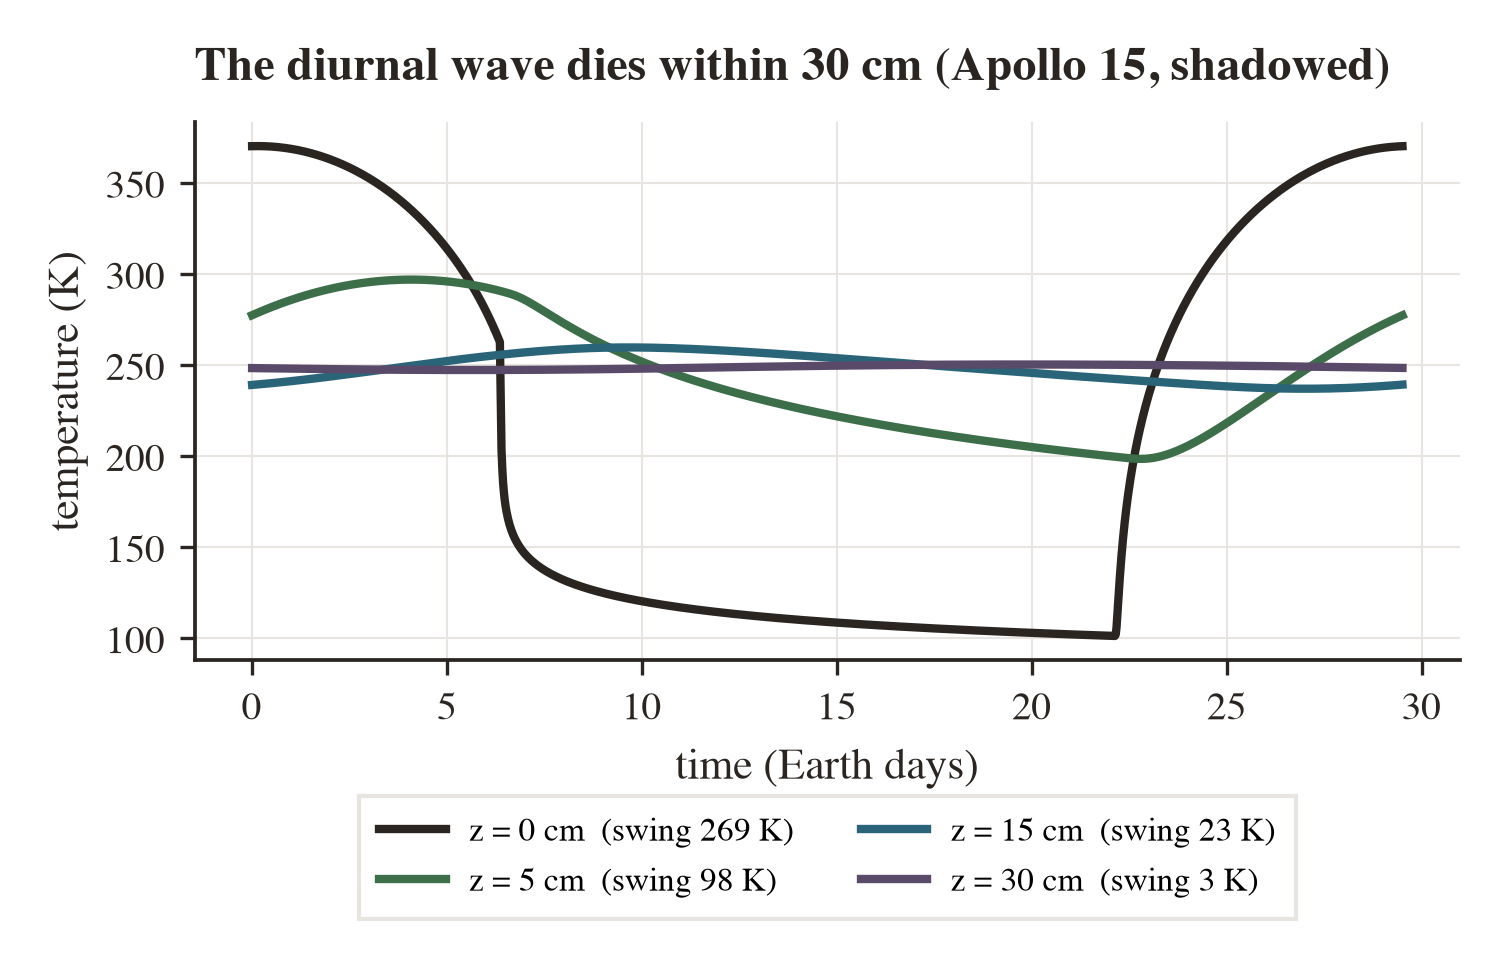
\includegraphics[width=0.66\linewidth]{aogs_wave_decay.pdf}
  \caption{The diurnal temperature wave decays within the top $\sim$10--20 cm. Below
  it, only the mean profile remains --- the quantity the deep sensors sample and the
  model predicts.}
  \label{fig:wave}
\end{figure}

Naively, finding the equilibrium means time-stepping Equation~\eqref{eq:heat} for
thousands of lunations until it stops drifting --- very slow. Instead the solver uses
a \textbf{flux-anchored closure}. In steady periodic state the cycle-mean heat flux
must equal $Q_b$ at every depth. If conductivity were constant this would just say
$d\overline{T}/dz = Q_b/K$. But $K$ depends on temperature, and the surface swing is
large, so there is a subtlety: because $K$ rises with $T$, the column conducts heat
\emph{downward} more efficiently during the hot part of the cycle than it conducts it
back up during the cold part. This leaves a small net downward ``rectified'' flux
$u_{\rm rect}$ in the upper regolith. The correct mean-gradient law is therefore
\begin{equation}
  \frac{d\overline{T}}{dz} \;=\; \frac{Q_b - u_{\rm rect}(z)}{K(\overline{T},z)},
  \qquad u_{\rm rect} = \big\langle K(T)\,\partial_z T\big\rangle - K(\overline{T})\,\partial_z\overline{T}.
  \label{eq:closure}
\end{equation}

\begin{intuition}
\intro Sign matters: it is \emph{minus} $u_{\rm rect}$. The day--night nonlinearity
quietly pumps a bit of heat downward, stealing it from the mean gradient. The solver
anchors the mean temperature at $z_0 = 55$ cm --- deep enough that this rectification
is spent ($<1\%$ of $Q_b$) --- and integrates Equation~\eqref{eq:closure} outward.
This makes one equilibrium solve take $\sim$0.6 s instead of minutes, which is what
makes a 650-configuration sweep feasible. On this study's winners the flux budget
closes to $\le\closurewin\%$ and the anchor drifts $\le\driftmax$ mK.
\end{intuition}

% ════════════════════════════════════════════════════════════════════════════
\shead{3\enspace Advance 1 --- topographic shadowing}
This is the part you asked to see spelled out. It has four moving pieces: the
elevation map, the horizon each site sees, the Sun's path, and the rule that blocks
the beam. Then a fifth --- the terrain's \emph{warming} channel --- completes the
picture.

\sub{3.1\enspace The digital elevation model (DEM)}
A DEM is a grid of ground heights. We use the LOLA (Lunar Orbiter Laser Altimeter)
global model at \textbf{16 pixels per degree}, i.e.\ $\approx$1.9 km per pixel at the
equator. The file is a raw 16-bit height array; the code memory-maps it and reads
only the handful of points each ray needs, so a multi-gigabyte global map never
loads into RAM. Height is stored as an integer ``digital number'' converted to
kilometres by a fixed scale (0.5 m per count). Figure~\ref{fig:sites} shows the two
sites on the DEM with the skylines derived below.

\begin{intuition}
\intro Picture a giant elevation spreadsheet of the whole Moon: each cell is a
1.9-km square holding one height. To find a site's skyline we read heights outward
from the borehole along many compass directions.
\end{intuition}

\sub{3.2\enspace The horizon algorithm, step by step}
\label{sec:horizon}
The goal is the \textbf{skyline}: for every compass direction (azimuth), the
elevation angle of the highest terrain in that direction. If the Sun sits below that
angle, the site is in shadow. The code (\texttt{horizon\_profile}) does this by
\emph{ray casting}:

\begin{enumerate}
  \item \textbf{Pick 90 azimuths} evenly around the compass ($N_{\rm az}=90$, i.e.\
    one ray every $4^\circ$), measured from North, going East.
  \item \textbf{March each ray outward} in steps of one DEM pixel (capped at 1 km),
    out to $r_{\max}=150$ km. At range $r$ along azimuth $a$, the sample point's
    offset from the site $(\varphi_0,\lambda_0)$ on the sphere of radius
    $R_{\mathrm{M}}=1737.4$ km is
    \[
      \Delta\varphi = \frac{r}{R_{\mathrm{M}}}\cos a,\qquad
      \Delta\lambda = \frac{r}{R_{\mathrm{M}}}\frac{\sin a}{\cos\varphi_0}
    \]
    (converted to degrees). Read the terrain height $h(r)$ there by bilinear
    interpolation of the DEM.
  \item \textbf{Subtract the curvature drop.} The Moon is a sphere, so a point a
    distance $r$ away sits \emph{below} the local horizontal plane by
    \begin{equation}
      \mathrm{drop}(r) \;=\; \frac{r^2}{2R_{\mathrm{M}}}.
      \label{eq:drop}
    \end{equation}
    (At 150 km this is $150^2/(2\cdot1737.4)\approx6.5$ km --- not negligible.)
  \item \textbf{Elevation angle to each sample.} With the site height $h_0$,
    \begin{equation}
      \theta(r) \;=\; \arctan\!\frac{h(r) - h_0 - \mathrm{drop}(r)}{r}.
      \label{eq:elev}
    \end{equation}
    A positive $\theta$ means that terrain pokes above the site's horizontal.
  \item \textbf{The horizon is the maximum} along the ray,
    $\theta_h(a) = \max_r \theta(r)$, floored at $0$ (a flat or dished horizon is
    treated as flat). The \emph{first} obstacle is not necessarily the horizon --- a
    tall distant massif can out-top a low near ridge, which is why we take the max
    over the whole ray, not the nearest hit.
  \item Repeat for all 90 azimuths $\Rightarrow$ the skyline $\theta_h(a)$.
\end{enumerate}

\begin{worked}
\workedhdr One ray at Apollo 15, toward the Apennine front. Suppose 25 km out the
DEM shows terrain 2.0 km higher than the site. The curvature drop there is
$25^2/(2\cdot1737.4)=0.18$ km, so the effective rise is $2.0-0.18=1.82$ km over a
25 km run: $\theta=\arctan(1.82/25)=4.2^\circ$. A closer 5-km ridge only 0.25 km
tall gives $\arctan(0.25/5)=2.9^\circ$ --- lower, so the distant front wins and sets
the horizon in that direction. Sweeping all rays, Apollo 15's tallest horizon
reaches $\horAfif^\circ$; Apollo 17's, hard against the North Massif, reaches
$\horAsev^\circ$.
\end{worked}

\begin{figure}[H]\centering
  \includegraphics[width=0.98\linewidth]{poster_sites.pdf}
  \caption{The two sites on the LOLA DEM (top) and their ray-traced skylines
  (bottom, polar plots: angle = azimuth, radius = horizon elevation). Apollo 15 sits
  under the Apennine front; Apollo 17 is ringed by the Taurus--Littrow massifs. The
  dotted curve is the Sun's path (\S\ref{sec:suntrack}); where it dips under the
  skyline, the site is shadowed.}
  \label{fig:sites}
\end{figure}

\sub{3.3\enspace The Sun's path across the sky}
\label{sec:suntrack}
We need to know where the Sun is at each moment to test it against the skyline. The
Moon's spin axis is nearly perpendicular to its orbit (obliquity $\sim1.5^\circ$), so
to excellent approximation the sub-solar point sits on the equator (declination
$0$). With hour angle $h = 2\pi t / T_{\rm lunar}$ (noon at $t=0$,
$T_{\rm lunar}=29.53$ days), the Sun's elevation $e$ and azimuth $A$ at latitude
$\varphi$ are
\begin{equation}
  \sin e = \cos\varphi\,\cos h, \qquad
  A = \operatorname{atan2}(-\sin h,\; -\sin\varphi\,\cos h).
  \label{eq:sun}
\end{equation}
Over one lunation this traces a shallow arc: the Sun climbs from the eastern horizon,
peaks near elevation $90^\circ-\varphi$ at local noon, and sets in the west.

\sub{3.4\enspace Blocking the beam}
Now combine skyline and Sun (\texttt{shadowed\_insolation}). At each time $t$:
interpolate the horizon at the Sun's current azimuth, $\theta_h(A(t))$, and compare:
\begin{equation}
  S_{\rm sh}(t) \;=\;
  \begin{cases}
    S_0\sin e(t), & e(t) > \theta_h(A(t)) \quad\text{(Sun above the skyline: lit)}\\[2pt]
    0, & e(t) \le \theta_h(A(t)) \quad\text{(Sun behind terrain: blocked)}
  \end{cases}
  \label{eq:shadow}
\end{equation}
This $S_{\rm sh}(t)$ is precisely the forcing that enters the surface balance,
Equation~\eqref{eq:surf}. Figure~\ref{fig:forcing} shows the result: the standard
flat-site insolation with bites taken out of its sunrise and sunset edges, where the
Sun is low and the terrain intercepts it.

\begin{figure}[H]\centering
  \includegraphics[width=0.80\linewidth]{poster_forcing.pdf}
  \caption{Insolation over a lunation: the flat-site curve (grey) versus the
  DEM-shadowed curve. Shadowing removes the low-Sun ``horns'' at dawn and dusk ---
  the first and last slice of every lunar day.}
  \label{fig:forcing}
\end{figure}

\sub{3.5\enspace Why a 1\% energy loss is a first-order effect}
\label{sec:timing}
Integrated over a lunation, shadowing removes only \lossAfif\% of the sunlight at
Apollo 15 and \lossAsev\% at Apollo 17 --- tiny. Yet it cools the \emph{deep mean}
temperature by \shadowcoolAfif\ K (A15) and \shadowcoolAsev\ K (A17), which is the
same order as the misfit the whole study is explaining. How can 1\% of the energy
move the answer by kelvins?

\begin{intuition}
\intro Because \emph{when} the light is removed matters more than \emph{how much}.
Shadowing strikes at dawn and dusk, when the Sun is low. At those moments the
surface is coolest, and --- crucially --- the radiative conductivity term ($\propto
T^3$) is weakest, so the column is least able to buffer the loss. Removing energy
exactly when the ground is coldest biases the whole time-average downward far more
than the raw percentage suggests. This is the same rectification idea as
\S\ref{sec:closure}, seen from the forcing side.
\end{intuition}

\sub{3.6\enspace The terrain also warms: the second channel}
\label{sec:svf}
Blocking the direct beam is only half the story. The same hills that block the Sun
also \emph{fill part of the sky}, and warm terrain radiates infrared back at the
site (and bounces some sunlight back too). We quantify the open sky with the
\textbf{sky-view factor}
\begin{equation}
  \mathrm{SVF} \;=\; \big\langle \cos^2\theta_h \big\rangle_{\rm azimuth},
  \qquad \mathrm{SVF} = \svfAfif~(\mathrm{A15})\,/\,\svfAsev~(\mathrm{A17}).
  \label{eq:svf}
\end{equation}
The complement $(1-\mathrm{SVF})\approx1$--$1.5\%$ is the fraction of the sky filled
by terrain. Two warming effects follow, both scaling with $(1-\mathrm{SVF})$:
\begin{itemize}
  \item \textbf{Infrared self-heating.} With terrain at roughly the surface
    temperature ($T_{\rm terr}\approx T_s$, an upper bound), the site radiates to a
    partly-warm sky rather than cold space. This is an \emph{effective emissivity}
    $\varepsilon_{\rm eff}=\varepsilon[1-\varepsilon(1-\mathrm{SVF})]$ --- the column
    loses slightly less heat and warms.
  \item \textbf{Reflected sunlight.} Terrain visible over $(1-\mathrm{SVF})$ reflects
    $A\,S$ back onto the site.
\end{itemize}
Together these warm the deep sensors by $+\svfdtallAfif$ K (A15) and
$+\svfdtallAsev$ K (A17). So topography \textbf{enters twice}, through opposing
channels of comparable size: cooling by shadow (\shadowcoolAfif/\shadowcoolAsev\ K)
versus warming by terrain ($+\svfdtallAfif/+\svfdtallAsev$ K). At Apollo 15 cooling
wins; at Apollo 17 they nearly cancel. Neither can be dropped on the assumption that
the other erases it.

\begin{intuition}
\intro Honest caveat to state up front: the warming numbers are an \emph{upper
bound} (they assume the terrain is as warm as the sunlit surface), and they are a
\emph{diagnostic} --- they were computed after the main sweep, not folded into it.
The shadow-cooling numbers \emph{are} in the sweep. So ``topography is first-order''
is firmly true at Apollo 15; at Apollo 17 the net is small and depends on the
terrain-temperature assumption.
\end{intuition}

% ════════════════════════════════════════════════════════════════════════════
\shead{4\enspace Advance 2 --- discrete density layers and the grid}
The second addition replaces Hayne's one smooth density curve with a three-layer
staircase, and --- the key move --- lets density act on \emph{conductivity}, not just
heat storage.

\sub{4.1\enspace Why layers at all}
Hayne's density profile is a smooth exponential from a loose surface
($\rho_s=1100$ kg\,m$^{-3}$) to a compact deep value ($\rho_d=1800$), with globally
fixed endpoints. Real regolith, sampled in the Apollo drive cores, looks more like
\emph{distinct strata}: a loose skin, a transition, and consolidated material, with
the compaction happening within the first few tens of centimetres. A three-layer
model is the coarsest description that can hold that structure.

\sub{4.2\enspace The three-layer parameterization}
The density profile is a step function,
\begin{equation}
  \rho(z) =
  \begin{cases}
    \rho_1, & z < z_1 \quad\text{(surface skin)}\\
    \rho_2, & z_1 \le z < z_2 \quad\text{(intermediate)}\\
    \rho_3, & z \ge z_2 \quad\text{(consolidated deep)}
  \end{cases}
  \label{eq:rho3}
\end{equation}
--- five numbers: two boundary depths $z_1,z_2$ and three densities
$\rho_1\le\rho_2\le\rho_3$.

\sub{4.3\enspace The two branches: what density is allowed to change}
\label{sec:branches}
This is the crux of the whole study, and it is a \emph{controlled experiment}. When
we change a layer's density, we can let it affect the physics in two different ways:

\begin{itemize}
  \item \textbf{cp branch.} Density enters only the volumetric heat capacity
    $\rho\,c_p$ in Equation~\eqref{eq:heat} --- how much heat the layer stores.
    Conductivity is held at the certified $K_d^{\star}$. \emph{Density changes
    thermal inertia only.}
  \item \textbf{coupled branch.} Density \emph{also} sets the contact conductivity,
    because in Hayne's own model $K_c$ and $\rho$ share the same depth kernel. Write
    both as exponentials with the same $e^{-z/H}$ and eliminate it:
    \[
      K_c(z) = K_d - (K_d-K_s)e^{-z/H}, \quad
      \rho(z) = \rho_d - (\rho_d-\rho_s)e^{-z/H}
      \;\Longrightarrow\;
    \]
    \begin{equation}
      \boxed{\,K_c(\rho) \;=\; K_d - (K_d - K_s)\,\frac{\rho_d - \rho}{\rho_d - \rho_s}\,}
      \label{eq:kcrho}
    \end{equation}
    a straight line in $\rho$ pinned to $(\rho_s,K_s)$ and $(\rho_d,K_d^{\star})$.
    So a chosen layer density $\rho_3$ implies a conductivity
    $K_c(\rho_3)$ --- \emph{no new constants are introduced}.
\end{itemize}

\begin{intuition}
\intro Two doors for density. Through the ``cp'' door it only changes how much heat
the ground banks; through the ``coupled'' door it also changes how fast heat flows.
Running both and comparing tells you \emph{which} property the Apollo data actually
cares about. Spoiler (Part~V): the conductivity door does almost all the work.
\end{intuition}

\begin{worked}
\workedhdr What conductivity does a deep density of 1900 imply at Apollo 17? Use
Equation~\eqref{eq:kcrho} with $K_s=0.74$, $\rho_s=1100$, $\rho_d=1800$,
$K_d^{\star}=\kdstarAsev$:
\[
  K_c(1900) = 7.08 - (7.08-0.74)\frac{1800-1900}{1800-1100}
            = 7.08 - 6.34\cdot(-0.143) = 7.99~\mathrm{mW\,m^{-1}K^{-1}}.
\]
So the coupled winner's \emph{effective} deep conductivity is 7.99, above the anchor
$7.08$ --- the layer is denser than Hayne's $\rho_d$, so the line extrapolates
slightly past it. Hold onto this number; it is the heart of the degeneracy in
\S\ref{sec:degeneracy}.
\end{worked}

\begin{figure}[H]\centering
  \includegraphics[width=\linewidth]{aogs_cp_vs_coupled.pdf}
  \caption{The two branches, side by side. \emph{Left:} density does two jobs ---
  it changes heat storage ($\rho c_p$) and conductivity ($K_c$). The \textbf{cp}
  branch uses only the storage job (conductivity frozen at $K_d^{\star}$); the
  \textbf{coupled} branch uses both. \emph{Right:} the actual coupling line,
  Equation~\eqref{eq:kcrho} --- a denser layer reads a higher conductivity off the
  solid line (anchored at Hayne's two endpoints, open circles), while cp ignores
  density and stays on the dashed line. The right panel \emph{is} the equation the
  coupled branch applies.}
  \label{fig:cpcoupled}
\end{figure}

\sub{4.4\enspace The grid: how each value was chosen}
\label{sec:grid}
We do not know the true five numbers, so we sweep a grid and score every combination.
The grid is small but every value is bounded by real data, not guessed:

\begin{center}\small
\begin{tabular}{@{}llp{8.4cm}@{}}
\toprule
knob & values swept & justification\\
\midrule
$\rho_1$ & 1100, 1300, 1500 & Surface layer. \textbf{1100} is exactly Hayne's
  loosest surface value $\rho_s$ (the fluffiest plausible skin); the upper end
  brackets a moderately compacted skin.\\
$\rho_2$ & 1500, 1700 & Intermediate layer, between skin and deep.\\
$\rho_3$ & 1700, 1800, 1900 & Deep layer. \textbf{1800} is Hayne's $\rho_d$; 1900
  reaches toward the compacted bulk densities \emph{measured} in the Apollo drive
  cores ($\sim$1825/1960 kg\,m$^{-3}$; Grott et al.). Real regolith does not exceed
  this range.\\
$z_1$ & 5, 10, 20 cm & Skin$\to$intermediate boundary. Brackets the few-cm-to-
  decimetre scale of the loosest fluff (Hayne's $H=6$ cm sits inside it).\\
$z_2$ & 30, 50, 80 cm & Intermediate$\to$deep boundary. Brackets the depth at which
  cores show consolidation --- but stays \emph{above} the deep sensors (0.8--2.4 m)
  so the sensors can feel the structure.\\
\bottomrule
\end{tabular}
\end{center}

\noindent\textbf{Two rules prune and size the grid:}
\begin{enumerate}
  \item \textbf{Monotonicity} $\rho_1\le\rho_2\le\rho_3$: regolith compacts under its
    own overburden, so density can only rise (or stay) with depth --- an inverted
    profile is unphysical. Of the $3\times2\times3=18$ raw density combinations, all
    18 happen to satisfy this (because $\max\rho_1=\min\rho_2$ and
    $\max\rho_2=\min\rho_3$), giving \textbf{18 valid density triples}.
  \item Each triple is combined with every $(z_1,z_2)$ pair: $3\times3=9$. So
    $18\times9 = \mathbf{162}$ profiles per site per branch, and with both branches
    and the two sites the study runs \textbf{650 configurations} in total (162
    coupled $+$ 162 cp per site, plus the continuous-Hayne baselines).
\end{enumerate}

\begin{figure}[H]\centering
  \includegraphics[width=\linewidth]{aogs_combinations.pdf}
  \caption{How the count works. Each of the five knobs has 2--3 allowed values; the
  three densities multiply to 18 valid triples (all obey the denser-with-depth rule,
  because the grids overlap at 1500 and 1700), the two boundary depths to 9 pairs, and
  $18\times9=162$ profiles per site. Run over both branches and both sites (plus two
  baselines) gives the 650 runs of the full study.}
  \label{fig:combos}
\end{figure}

\begin{intuition}
\intro The grid is a coarse net cast only over structures the Moon actually allows:
densities between ``Hayne's fluff'' and ``measured drive-core compaction,'' getting
denser with depth, compacting somewhere above the sensors. It is deliberately small
and physical rather than a large blind optimization --- which also keeps the
overfitting risk down (\S\ref{sec:overfit}).
\end{intuition}

\begin{figure}[H]\centering
  \includegraphics[width=0.98\linewidth]{poster_density_sweep.pdf}
  \caption{The search made visible. Every one of the 162 swept coupled profiles is
  drawn as a density staircase and shaded by its deep-sensor RMSE (dark = best fit).
  Bold = the winning profile; dotted = Hayne's smooth continuous model. Both sites
  prefer a surface denser than Hayne and a compaction step high in the column.}
  \label{fig:sweep}
\end{figure}

% ════════════════════════════════════════════════════════════════════════════
\shead{5\enspace Retrieval, the degeneracy, and the results}

\sub{5.1\enspace Scoring a profile}
For each of the 162 profiles per branch: build $\rho(z)$ (and, in the coupled
branch, $K_c(\rho)$), solve for the periodic-equilibrium mean profile
$\overline{T}(z)$ using the flux-anchored solver of \S\ref{sec:closure}, sample it at
the Apollo sensor depths, and compute the misfit
\begin{equation}
  \mathrm{RMSE} = \sqrt{\big\langle(\overline{T}(z_i) - T_i^{\rm obs})^2\big\rangle_i}
  \quad\text{over the deep sensors } (0.8\text{--}2.4~\mathrm{m}).
  \label{eq:rmse}
\end{equation}
We score only the \emph{deep} sensors: the shallow thermocouples sit in or near the
borestem and are perturbed by drilling and by conduction down the stem, so Langseth's
own analysis treats them separately. The deep sensors sit below the diurnal skin and
cleanly sample the mean gradient the model predicts. One equilibrium temperature per
sensor is taken from quiet late-mission windows of the 1971--77 record (the 1975--77
portion restored by Nagihara et al.\ 2018).

\sub{5.2\enspace The degeneracy you must understand}
\label{sec:degeneracy}
The deep temperature gradient is essentially $Q_b/K_{\rm deep}$. \emph{Both} a higher
deep conductivity $K_d$ \emph{and} a denser deep layer (which raises $K_c(\rho)$)
increase $K_{\rm deep}$ --- and they produce the \emph{same} gradient. So the sensors
alone cannot separate ``more conductive'' from ``denser.''

\begin{intuition}
\intro One measurement (the deep slope), two knobs that both control it. You can
trade a higher $K_d$ for a lighter deep layer and get an identical fit. The letter
resolved this by \emph{fixing} density (to Hayne) and solving for $K_d^{\star}$; this
study \emph{fixes} $K_d^{\star}$ and solves for density. They are two conditional
slices of one coupled $(K_d,\rho)$ space --- not a contradiction, and not independent
facts. This is why the coupled winner's effective deep conductivity is
$K_c(\rho_3)$, not $K_d^{\star}$: at Apollo 17, $\rho_3=1900$ gives 7.99, not 7.08
(the worked example of \S4.3). The fully rigorous version --- retrieving $K_d$ and
$\rho$ \emph{jointly} with a density prior --- is the identified next step.
\end{intuition}

\begin{figure}[H]\centering
  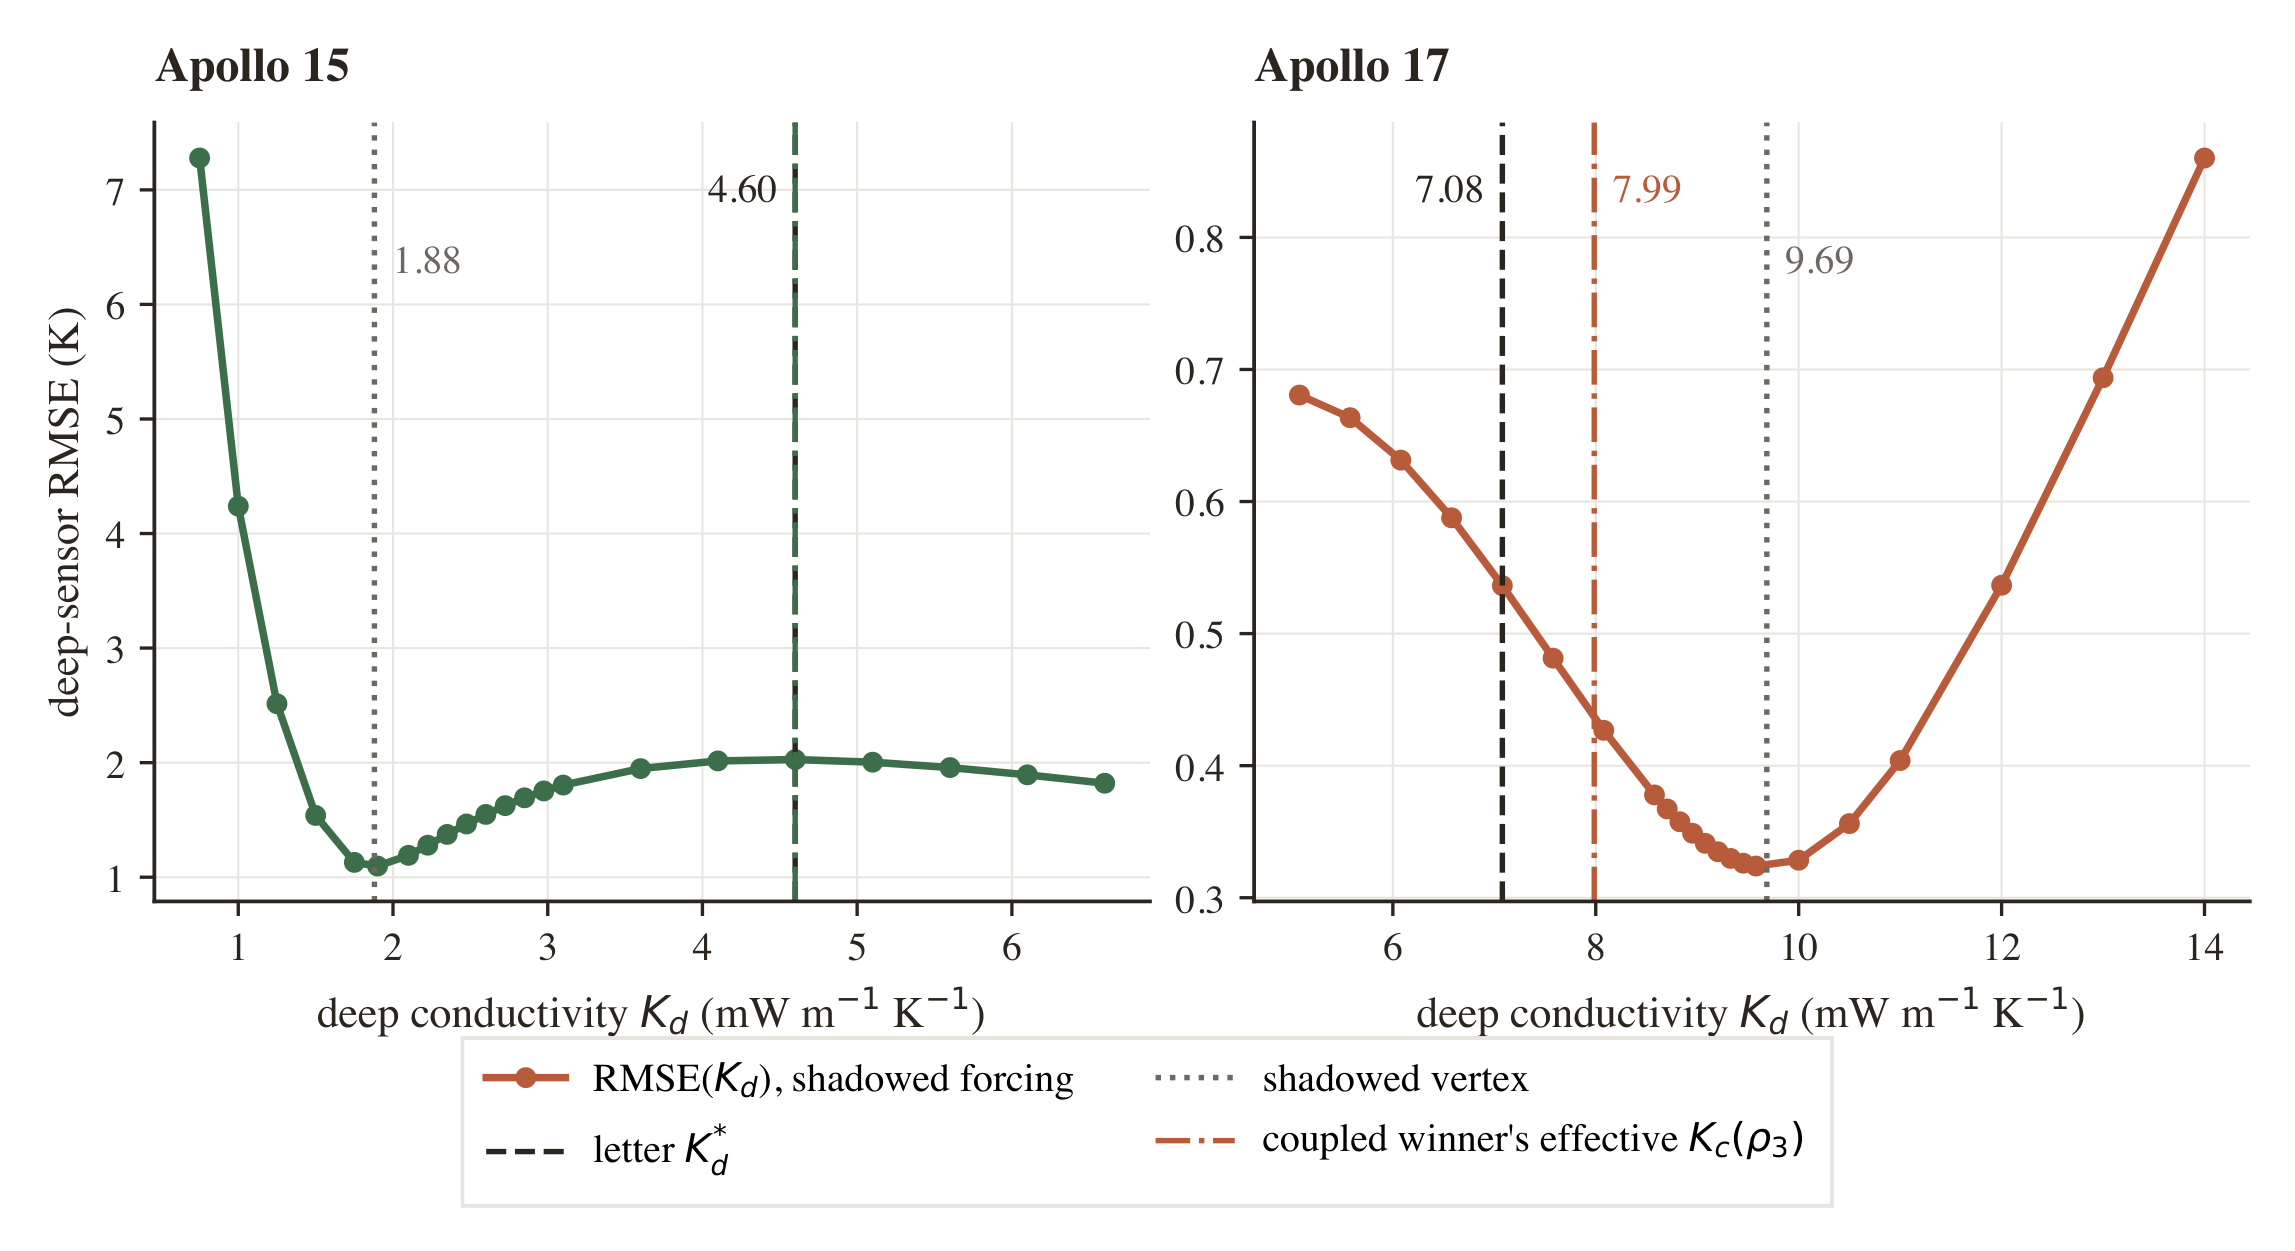
\includegraphics[width=0.82\linewidth]{explainer_kd_bowl.pdf}
  \caption{The degeneracy drawn. The retrieval ``bowl'' in $K_d$ under shadowed
  forcing: dashed = the letter's $K_d^{\star}$; dash-dot = the coupled winner's
  effective deep conductivity $K_c(\rho_3)$. At Apollo 15 they coincide (its winner's
  deep density equals Hayne's); at Apollo 17 the winner sits above $K_d^{\star}$ ---
  the trade-off, made visible.}
  \label{fig:bowl}
\end{figure}

\sub{5.3\enspace What the data say}
The winners and the model-class ladder are in Table~\ref{tab:ladder} and
Figure~\ref{fig:profiles}. Three readings:
\begin{itemize}
  \item \textbf{Layering reproduces the record.} The best coupled columns fit the
    deep sensors to \rmsecKAfif\ K (A15) and \rmsecKAsev\ K (A17) --- a factor
    $\sim$2.6 (A15) and $\sim$10 (A17) better than a homogeneous column, and
    $\sim$2.3 / $\sim$1.5 better than Hayne's continuous model (the honest,
    field-standard comparison).
  \item \textbf{The lever is conductivity, not heat capacity.} Across the whole
    sweep the cp branch moves the fit by $<0.8$ K; the coupled branch spans $\sim$4 K
    (Figure~\ref{fig:sens}). Density matters through the conductivity it implies.
  \item \textbf{The structure is physical, not fitted.} Retrieved deep densities
    (1800/1900) match the drive cores in magnitude and site ordering, and a
    structure transplanted to the \emph{other} site still beats homogeneous
    (Figure~\ref{fig:transfer}).
\end{itemize}

\begin{table}[H]\centering\small
\caption{Deep-sensor RMSE (K) by model class, under shadowed forcing.}
\label{tab:ladder}
\begin{tabular}{lcc}
\toprule
model & A15 & A17\\
\midrule
homogeneous (constant $K$, constant $\rho$)     & \rmsehomAfif & \rmsehomAsev\\
Hayne continuous at site $K_d^{\star}$          & \rmsehayAfif & \rmsehayAsev\\
best cp (density $\to$ heat capacity)           & \rmsecpAfif  & \rmsecpAsev\\
best coupled (density $\to$ conductivity)       & \textbf{\rmsecKAfif} & \textbf{\rmsecKAsev}\\
\bottomrule
\end{tabular}
\end{table}

\begin{figure}[H]\centering
  \includegraphics[width=0.72\linewidth]{poster_profiles.pdf}
  \caption{Validation. Modeled mean temperature at the sensor depths vs the Apollo
  deep sensors (circles). The heat-capacity-only branch can shift the deep profile
  but not \emph{tilt} it; the density-coupled branch tilts the gradient onto the
  measurements --- which is why it succeeds where the smooth models miss.}
  \label{fig:profiles}
\end{figure}

\begin{figure}[H]\centering
  \includegraphics[width=0.62\linewidth]{poster_sens.pdf}
  \caption{Sensitivity. \emph{Top:} RMSE spread over all configurations --- cp tight
  ($<0.8$ K), coupled wide ($\sim$4 K): the conductivity channel is the lever.
  \emph{Bottom:} RMSE over the boundary-depth plane; green (good) sits at a shallow
  consolidation depth $z_2=30$ cm (Apollo 17 also admits a tied deeper solution).}
  \label{fig:sens}
\end{figure}

\begin{figure}[H]\centering
  \includegraphics[width=0.52\linewidth]{poster_transfer.pdf}
  \caption{Cross-site transfer. Each site's retrieved structure scored at both sites.
  The diagonal is the home fit; the off-diagonal transplants the structure --- it
  degrades gracefully and still beats homogeneous, evidence the layering tracks
  geology rather than curve-fitting freedom.}
  \label{fig:transfer}
\end{figure}

\sub{5.4\enspace How robust is it? The bootstrap}
\label{sec:overfit}
Five swept parameters against $\sim$a dozen sensor temperatures raises a fair
overfitting worry. Three things address it. First, the cp branch is a built-in
\emph{null experiment}: identical parameter freedom, but with the conductivity
channel switched off it barely moves --- so the freedom alone does not manufacture
the fit. Second, cross-site transfer (Figure~\ref{fig:transfer}) is a held-out test.
Third, a \textbf{10{,}000-draw bootstrap} resamples the sensors and their
uncertainties and re-scores; the best-RMSE 95\% confidence intervals of both branches
stay entirely below the homogeneous baseline at both sites (coupled
\bootcicKAfif/\bootcicKAsev\ K).

\begin{intuition}
\intro What the bootstrap does \emph{not} do: it resamples sensor noise, not model
choice. And it tells us the exact best A15 triple is fragile --- it survives only
\stabcKAfif\% of draws (A17's is sturdier at \stabcKAsev\%). So the honest claim is
the \emph{class} of profile (denser-than-Hayne surface, shallow consolidation), not
one exact triple. Always quote the class.
\end{intuition}

\begin{figure}[H]\centering
  \includegraphics[width=0.86\linewidth]{poster_bootstrap.pdf}
  \caption{Robustness. Best-RMSE 95\% confidence intervals from 10{,}000 bootstrap
  draws, both branches, both sites, against the homogeneous baseline (dashed / arrow
  where off-scale). The layered improvement is not an artefact of any single sensor.}
  \label{fig:bootstrap}
\end{figure}

% ════════════════════════════════════════════════════════════════════════════
\shead{6\enspace Caveats, and what comes next}
Stated plainly, so you can raise them before anyone else does:
\begin{itemize}
  \item \textbf{Terrain warming is a diagnostic upper bound}, computed with
    $T_{\rm terr}\approx T_s$ and not yet folded into the 650-config sweep. A re-sweep
    with both topographic channels active is the natural follow-up.
  \item \textbf{The DEM is coarse.} At 16 ppd ($\approx$1.9 km/px) the near-field
    massifs are undersampled. Re-tracing the horizons on SLDEM2015 ($\approx$59 m/px)
    shifts them in \emph{both} directions --- A15 to $13.6^\circ$/0.54\%, A17 to
    $14.1^\circ$/0.24\% --- so the poster's 16 ppd numbers are labelled
    resolution-limited. Propagating the finer DEM through the sweep is a drop-in
    next step.
  \item \textbf{$K_d$ and deep density are degenerate} from a single gradient
    (\S\ref{sec:degeneracy}); a joint $(K_d,\rho)$ retrieval with a density prior is
    the rigorous version.
  \item \textbf{$\chi$ and $Q_b$ are held fixed} at the certified values; in the
    parent error budget they dominate, so a full joint retrieval would vary them too.
\end{itemize}

\begin{intuition}
\intro The one-line ``so what.'' Landing-site thermal assessment must ray-trace
horizons \emph{and} count terrain radiation --- at the 1-K scale these are not
optional corrections, and both come free from a DEM. Density sensing through
conductivity works, verified here against the drive cores. And fifty-year-old Apollo
data still discriminates between modern model classes --- and is ready to calibrate
the next generation of in-situ heat-flow probes.
\end{intuition}

% ════════════════════════════════════════════════════════════════════════════
\shead{Appendix A\enspace Numbers at a glance}
\begin{center}\small
\begin{tabular}{@{}lcc@{}}
\toprule
 & \textbf{Apollo 15} & \textbf{Apollo 17}\\
\midrule
$K_d^{\star}$ anchor (mW\,m$^{-1}$K$^{-1}$) & \kdstarAfif & \kdstarAsev\\
best coupled RMSE (K) & \textbf{\rmsecKAfif} & \textbf{\rmsecKAsev}\\
best cp RMSE (K) & \rmsecpAfif & \rmsecpAsev\\
Hayne continuous RMSE (K) & \rmsehayAfif & \rmsehayAsev\\
homogeneous RMSE (K) & \rmsehomAfif & \rmsehomAsev\\
cross-site transfer RMSE (K) & \xferatAfif & \xferatAsev\\
best structure $\rho_{1,2,3}$ (kg\,m$^{-3}$) & \bestrhocKAfif & \bestrhocKAsev\\
best boundaries $z_1/z_2$ (cm) & \bestzcKAfif & \bestzcKAsev\\
bootstrap 95\% CI, coupled (K) & \bootcicKAfif & \bootcicKAsev\\
exact-winner stability & \stabcKAfif\% & \stabcKAsev\%\\
horizon max / insolation lost & \horAfif$^\circ$ / \lossAfif\% & \horAsev$^\circ$ / \lossAsev\%\\
shadow cooling at sensors (K) & \shadowcoolAfif & \shadowcoolAsev\\
terrain IR + reflected warming (K) & $+\svfdtallAfif$ & $+\svfdtallAsev$\\
SVF & \svfAfif & \svfAsev\\
$Q_b$ (mW\,m$^{-2}$) & 21 & 16\\
\bottomrule
\end{tabular}
\end{center}

\shead{Appendix B\enspace Where the code lives}
Everything is reproducible from the bundle at
\texttt{deliverables/documents/aogs/}:
\begin{itemize}
  \item \texttt{code/compute/s1\_sensitivity.py} --- the DEM loader, the horizon
    ray-caster (\texttt{horizon\_profile}), the Sun track (\texttt{sun\_track}), and
    the shadowed forcing (\texttt{shadowed\_insolation}) of Part~III.
  \item \texttt{code/compute/s2\_density\_study.py} --- the 3-layer grid, the two
    branches, and the $K_c(\rho)$ coupling of Part~IV; writes the 650-config archive.
  \item \texttt{code/compute/s6\_svf\_terms.py} --- the sky-view / terrain-radiation
    channel (\S\ref{sec:svf}).
  \item \texttt{code/compute/s7\_winner\_bootstrap.py} --- the robustness bootstrap.
  \item \texttt{code/make\_poster\_figures.py}, \texttt{make\_density\_sweep\_figure.py}
    --- regenerate every figure in this book.
  \item Companion documents: \texttt{aogs\_master\_overview.pdf} (figure-by-figure at
    a glance), \texttt{aogs\_expert\_briefing.pdf} (Q\&A for the session).
\end{itemize}

\vspace{6pt}{\color{teal}\rule{\linewidth}{0.9pt}}
\begin{center}\footnotesize\color{dim}
All physical values from the generated macros (\texttt{poster\_numbers.tex}) and the
results archives. Algorithm descriptions trace the actual code in
\texttt{code/compute/}.
\end{center}

\end{document}
